\chapter{Equazioni secondo grado}
\label{cha:equazioni2grado}
\minitoc
\mtcskip                                % put some skip here
\minilof                                % a minilof
\mtcskip                                % put some skip here
\minilot
\begin{figure}[H]
\centering
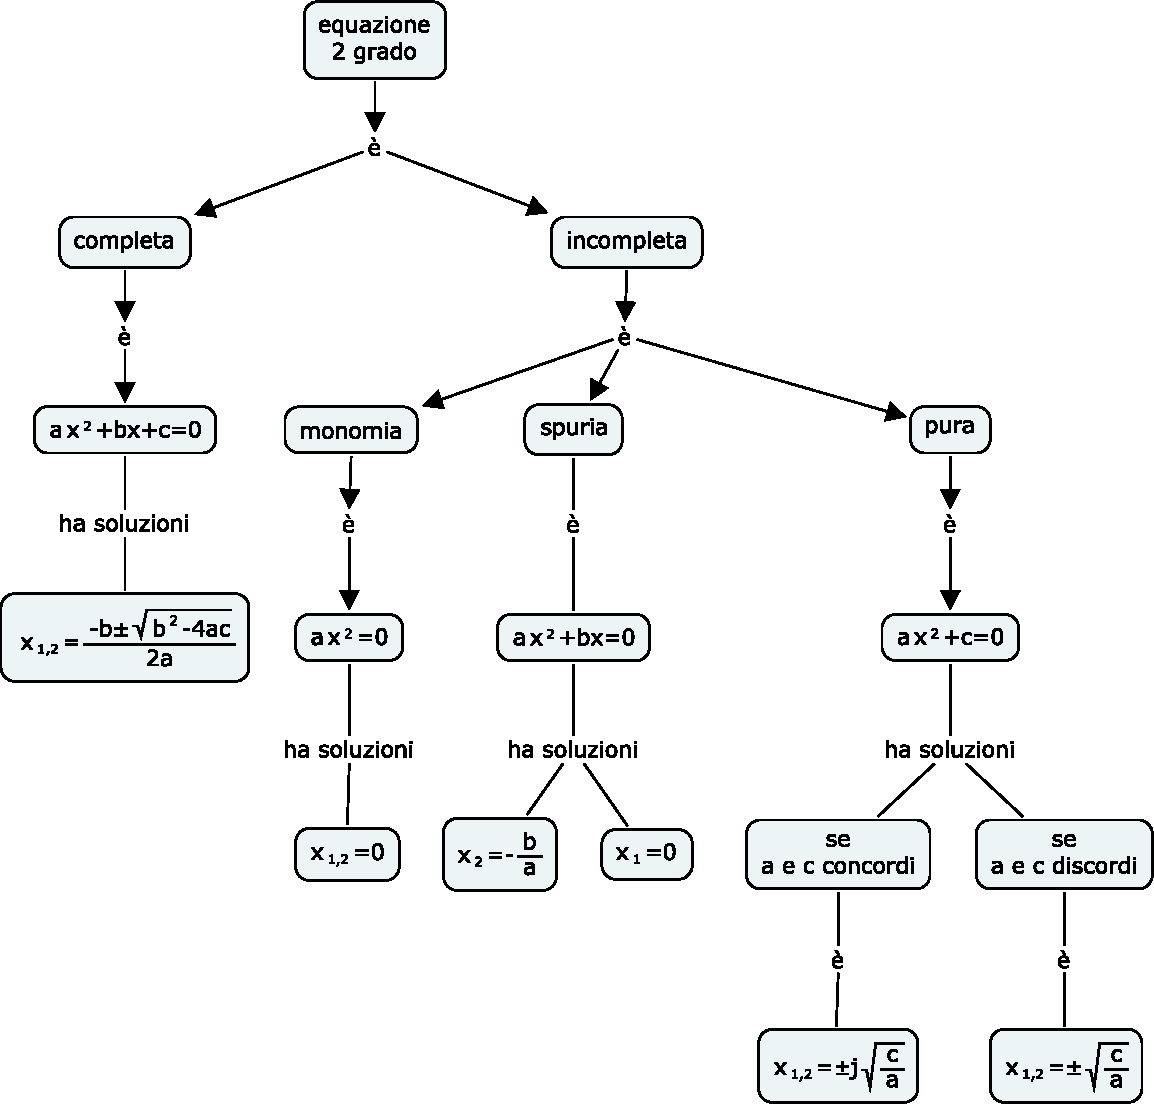
\includegraphics[scale=0.80]{equazioni2gradopdf-crop.pdf}
\caption{Equazioni secondo grado}
\label{fig:equazioni2gradocmap}
\end{figure}
\begin{table}[H]

\centering
\begin{tabular}{CCCCL}
\toprule
\multicolumn{5}{c}{ax=b}\\
\hline
%&\\
\multicolumn{2}{c}{coefficienti}&&soluzione&tipo soluzione\\
\midrule
a\neq0&b\neq0&ax=b&x=\dfrac{b}{a}&determinata\\
%&\\
a\neq0&b=0&ax=0&x=0&determinata\\
%&\\
a=0&b=0&0x=0&&indeterminata\\
%&\\
a=0&b\neq0&0x=b&&impossibile\\
\bottomrule	
\end{tabular}
\caption{Soluzioni equazioni primo grado intere}
\label{tab:equazioniprimogrado}
\end{table}
\begin{table}%

\centering
\begin{tabular}{LR}
\toprule
Tipo&Nome\\
\midrule
ax^2+c=0&Pura\\
\hline
\multicolumn{2}{c}{Risoluzione}\\
\multicolumn{2}{C}{ax^2=-c}\\
\multicolumn{2}{C}{x^2=-\dfrac{c}{a}}\\
\multirow{3}*{Se $-\dfrac{c}{a}>0$ esistono soluzioni reali} &x_1=-\sqrt{-\dfrac{c}{a}}\\
&\\
&x_2=+\sqrt{-\dfrac{c}{a}}\\
&\\
Se -\dfrac{c}{a}<0\text{ non esistono soluzioni reali}&\\
&\\
\bottomrule	
%\end{tabular}
%\caption{Equazione secondo grado pura}
%\label{tab:equazione2GradoPura}
%\end{table}
%\begin{table}%
%
%\centering
%\begin{tabular}{LR}
\toprule
Tipo&Nome\\
\midrule
ax^2+bx=0&Spuria\\
\hline
\multicolumn{2}{c}{Risoluzione}\\
\multicolumn{2}{C}{ax^2+bx=0}\\
\multicolumn{2}{C}{x(ax+b)=0}\\
\multicolumn{2}{C}{x_1=0}\\
\multicolumn{2}{C}{ax+b=0}\\
\multicolumn{2}{C}{x_2=-\dfrac{b}{a}}\\
\bottomrule	
%\end{tabular}
%\caption{Equazione secondo grado spuria}
%\label{tab:equazione2GradoSpuria}
%\end{table}
%\begin{table}%
%
%\centering
%\begin{tabular}{LR}
\toprule
Tipo&Nome\\
\midrule
ax^2=0&Monomia\\
\hline
\multicolumn{2}{c}{Risoluzione}\\
\multicolumn{2}{C}{ax^2=0}\\
\multicolumn{2}{C}{x_1=0}\\
\multicolumn{2}{C}{x_2=0}\\
\bottomrule	
%\end{tabular}
%\caption{Equazione secondo grado monomia}
%\label{tab:equazione2GradoMonomia}
%\end{table}
%\begin{table}%
%
%\centering
%\begin{tabular}{LR}
\toprule
Tipo&Nome\\%
\midrule
ax^2+bx+c=0&Completa\\%
\hline
\multicolumn{2}{c}{Risoluzione}\\%
\multirow{3}*{$b^2-4ac>0$}&x_1=\dfrac{-b+\sqrt{b^2-4ac}}{2a}\\%
&\\
&x_2=\dfrac{-b-\sqrt{b^2-4ac}}{2a}\\%
\hline
\multirow{3}*{$b^2-4ac=0$}&x_1=-\dfrac{b}{2a}\\%
&\\
&x_2=-\dfrac{b}{2a}\\%
\hline
\multirow{3}*{$b^2-4ac<0$}&\\
&\text{nessuna soluzione reale}\\%
&\\
\bottomrule	
\end{tabular}
\caption{Equazioni secondo grado}
\label{tab:equazione2Gradoelenco}
\end{table}
